% !TEX root = tracking.tex
\section{Offline Computations \label{sec:precomp}}
The offline computation begins with setting up a capture-avoid game between the tracking system and the planning system, which we then analyze using Hamilton Jacobi (HJ) reachability. In this game, the tracking system will try to "capture" the planning system, while the planning system is doing everything it can to avoid capture. In reality the planner may not actively be trying to avoid the tracking system, but this allows us to account for worst-case scenarios. If both systems are acting optimally in this way, we want to determine the largest relative distance that may occur over time. This distance is the maximum possible tracking error between the two systems. Note that this tracking error is independent of specific online paths; it depends only on relative states and dynamics.

\subsection{Relative Dynamics}
To determine the relative distance that may occur over time we must first define the relative states and dynamics between the tracking and planning models. The individual dynamics are defined in Section \ref{sec:formulation}. The relative system is found by fixing the planning model to the origin and finding the states of the tracking model relative to the planning model, as shown below.

\begin{equation}
\label{eq:rdyn}
\begin{aligned}
\rstate = \tstate - \ptmat\pstate\\
\dot\rstate = \rdyn(\rstate, \tctrl, \pctrl, \dstb)
\end{aligned}
\end{equation}

Matrix $\ptmat$ matches the common states of $\tstate$ and $\pstate$. The relative states $\rstate$ now represent the tracking states relative to the planning states.

\subsection{Formalizing the Capture-Avoid Game}
Now that we have the relative dynamics between the two systems we must define a metric for the tracking error bound between these systems. We do this by defining an implicit surface function as a cost function $\errfunc(\rstate)$ in the new frame of reference. Because the metric we care about is distance to the origin (and thus distance to the planner), this cost function can be as simple as distance in position space to the origin. An example can be seen in Figure \ref{fig:quad4D_example}-a, where the contour rings represent varying level sets of the cost function. The tracking system will try to minimize this cost to reduce the relative distance, while the planning system will do the opposite.

\begin{figure}
	\centering
	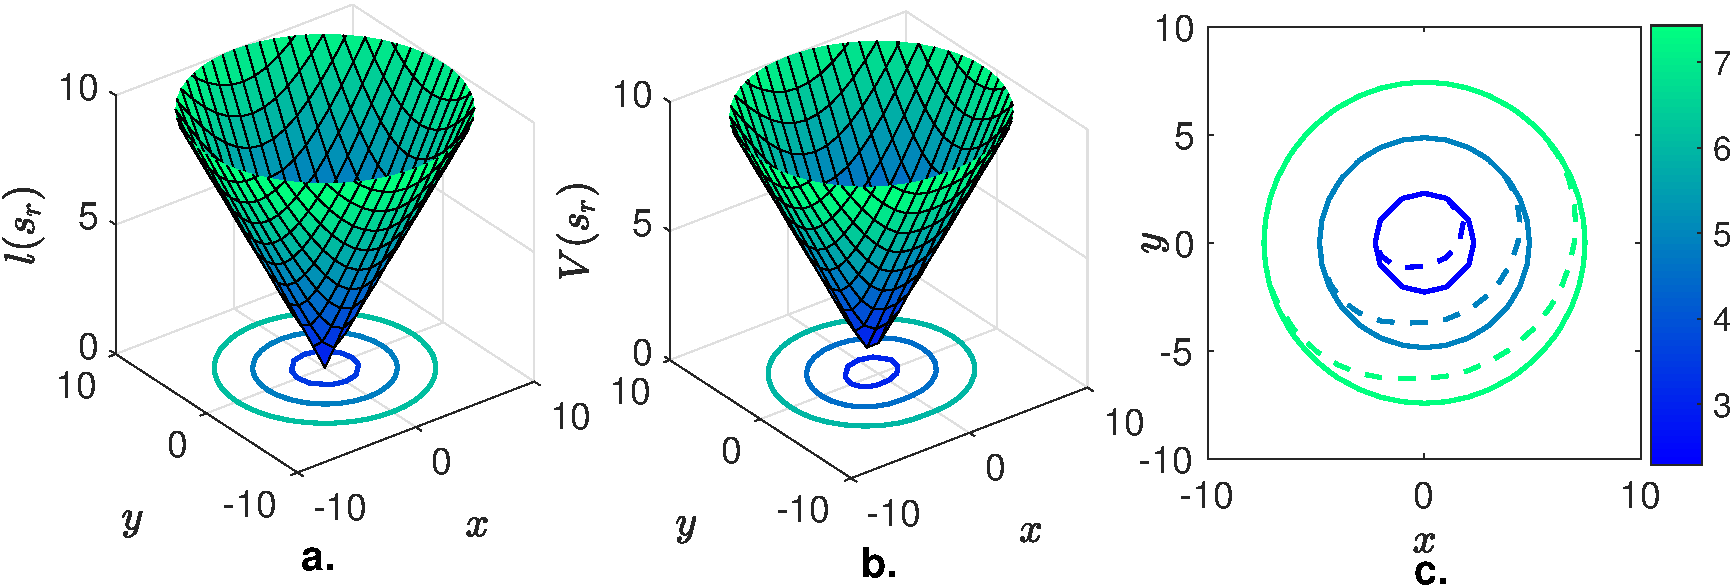
\includegraphics[width=0.5\textwidth]{fig/quad4D_example}
	\caption{illustrative example of the precomputation steps for a 4D quadrotor tracking a 2D kinematic planner. a) Cost Function defined on relative states, b) Value function computed using HJ reachability, c) Level sets of the cost function (solid) and value function (dashed). If the initial relative state is contained within the dashed set the system is guaranteed to remain within the solid set (i.e. the tracking error bound)}
	\label{fig:quad4D_example}
\end{figure} 
 
 We want to find the farthest distance (and thus highest cost) that this game will ever reach when both players are acting optimally. Therefore we want to find a mapping between the initial relative state of the system and the maximum possible cost achieved over the time horizon. This mapping is through our value function, defined as: \MCnote{Time horizon, time variable notation, control/disturbance functions, trajectory notation}
 \begin{equation}
 \begin{aligned}
 	V(\rstate)= \sup_{\pctrl(\cdot)} \inf_{\tctrl(\cdot), \dstb(\cdot)} \big\{\sup_{\tvar\in [0, \thor]} \errfunc(\rtraj(\tvar; \rstate, 0, \pctrl(\cdot), \tctrl(\cdot)))\big\}
 	\end{aligned}
 \end{equation} 
 
 This is a modified version of the Hamilton-Jacobi formulation as described by \textcolor{red}{cite jaime, time varying reachability}. By implementing HJ reachability analysis we solve for this value function over the time horizon. If the control authority of the tracking system is powerful enough to always eventually reach the planning system, this value function will converge to an invariant solution for all time. An example of this value function is in Figure \ref{fig:quad4D_example}-b. In the next section we will prove that the sub-level sets of this value function will map initial relative states to the guaranteed furthest possible tracking error over all time, as seen in Figure \ref{fig:quad4D_example}-c.
 
\subsection{Main Result}
 \begin{equation}
 \begin{aligned}
& \valfunc(\rstate, \thor) = \inf_{\pctrl(\cdot)} \sup_{\pctrl(\cdot), \dstb(\cdot)} \big\{\\
&\quad \max_{\tvar \in [0, \thor]} \errfunc(\rtraj(\tvar; \rstate, 0, \pctrl(\cdot), \pctrl(\cdot), \dstb(\cdot)))\big\} \\
& \valfunc(\rstate, \thor) = \max_{\tvar \in [0, \thor]} \errfunc(\rtraj^*(\tvar; \rstate, 0)) 
 \end{aligned}
  \end{equation}
 
 \begin{claim}
   \label{thm:main}
   Let $\thor_c \ge 0$, and suppose
   
   \begin{equation}
   \label{eq:conv_valfunc}
   \valfunc_\infty(\rstate) := \valfunc(\rstate, \thor) = \valfunc(\rstate, \thor_c) ~ \forall \thor \ge \thor_c.
   \end{equation}
   
   Then $\forall \tvar_1, \tvar_2$ with $\tvar_2 \ge \tvar_1$,
   
   \begin{equation}
   \label{eq:invariant}
   \valfunc_\infty(\rstate) \ge \valfunc_\infty\Big(\rtraj^*(\tvar_2;, \rstate, \tvar_1)\Big)
   \end{equation}
   
   \noindent where
   \begin{equation}
   \begin{aligned}
   & \rtraj^*(0;, \rstate, \tvar) := \rtraj(0; \rstate, \tvar, \pctrl^*(\cdot), \pctrl^*(\cdot), \dstb^*(\cdot))) \\
   & \pctrl^*(\cdot) = \arg \inf_{\pctrl(\cdot)} \sup_{\pctrl(\cdot), \dstb(\cdot)}\big\{ \\
   & \qquad \max_{\tvar \in [0, \thor]} \errfunc(\rtraj(0; \rstate, \tvar, \pctrl(\cdot), \pctrl(\cdot), \dstb(\cdot))) \big\}\\
   & \pctrl^*(\cdot) = \arg \sup_{\pctrl(\cdot)} \sup_{\dstb(\cdot)} \big\{ \\
   & \qquad \max_{t \in [0, \thor]} \errfunc(\rtraj(0; \rstate, \tvar, \pctrl(\cdot), \pctrl(\cdot), \dstb(\cdot))) \big\} \\
   & \dstb^*(\cdot) = \arg \sup_{\dstb(\cdot)} \big\{\max_{\tvar \in [0, \thor]} \errfunc(\rtraj(0; \rstate, \tvar, \pctrl(\cdot), \pctrl(\cdot),  \dstb(\cdot))) \big\}
   \end{aligned}
   \end{equation}
   
 \end{claim}
 
\textit{Proof:}

Assume $\thor \ge \thor_c$.

\begin{equation}
\begin{aligned}
\valfunc(\rstate, \thor) &= \valfunc_\infty(\rstate) = \max_{\tvar \in [0, \thor]} \errfunc(\rtraj^*(\tvar; \rstate, 0))\\
\end{aligned}
\end{equation}

By time-invariance
 \begin{equation}
 \begin{aligned}
 \valfunc_\infty(\rstate) &= \max_{\tvar \in [0, \thor]} \errfunc(\rtraj^*(\tvar; \rstate, 0)) \\
 &= \max_{\tvar \in [\thor_c-\thor, \thor_c]} \errfunc(\rtraj^*(\tvar; \rstate, \thor_c-\thor)) \\
 \end{aligned}
 \end{equation}  
 
Consider time subinterval:
 
 \begin{equation}
\begin{aligned}
\valfunc_\infty(\rstate) &= \max_{\tvar \in [0, \thor]} \errfunc(\rtraj^*(\tvar; \rstate, 0)) \\
&\ge \max_{\tvar \in [0, \thor_c]} \errfunc(\rtraj^*(\tvar; \rstate, \thor_c-\thor)) \\
\end{aligned}
\end{equation}  

Now look at trajectory $\rtraj^*(\tvar; \rstate, \thor_c-\thor)$:

\begin{equation}
\begin{aligned}
\rtraj^*(\tvar; \rstate, \thor_c-\thor) = \rtraj^*(\tvar; \rtraj^*(0; \rstate, \thor_c-\thor), 0)
\end{aligned}
\end{equation}

Continuing from value function:

\begin{equation}
\begin{aligned}
\valfunc_\infty(\rstate) &\ge \max_{\tvar \in [0, \thor_c]} \errfunc(\rtraj^*(\tvar; \rtraj^*(0; \rstate, \thor_c-\thor), 0)) \\
&= \valfunc_\infty(\rtraj^*(0; \rstate, \thor_c-\thor))
\end{aligned}
\end{equation} 
 
 By time-invariance again,
 
 \begin{equation}
 \begin{aligned}
 \valfunc_\infty(\rstate) &\ge \valfunc_\infty(\rtraj^*(\thor-\thor_c; \rstate, 0)) ~ \forall \thor\ge\thor_c \\
 \Leftrightarrow  \valfunc_\infty(\rstate) &\ge \valfunc_\infty(\rtraj^*(\tvar_2; \rstate, 0)) ~ \forall \tvar_2 \ge 0
 \end{aligned}
 \end{equation} 
 
   Since the system dynamics are time-invariant, we can pick $\tvar_2 = -\thor_c$ without loss of generality, and $\tvar_1 = -\thor$ to obtain the desired result. \hfill $\blacksquare$
 
\begin{rem}
  The interpretation of Theorem \ref{thm:main}, particularly \eqref{eq:invariant}, is that every level set of $\valfunc_\infty(\rstate)$ is invariant under the following conditions:
  \begin{itemize}
    \item The real system applies the optimal control which tries to track the virtual system;
    \item The virtual system applies the optimal virtual control that tries to escape from the real system;
    \item The real system experiences the worst-case disturbance.
  \end{itemize}
  
  In particular, the value of $\underline\valfunc := \valfunc_\infty(\rstate)$ can be interpreted as the smallest possible tracking error \MCnote{(we need to explicitly define tracking error)} given the above assumptions. The tracking error bound in Fig. \ref{fig:fw_online}, \ref{fig:hybrid_ctrl}, \ref{fig:fw_offline} is given by\footnote{In practice, since $\valfunc_\infty$ is obtained numerically, we set $\TEB = \{\rstate: \valfunc_\infty(\rstate) \le \underline\valfunc + \epsilon\}$ for some suitably small $\epsilon>0$} the set $\TEB = \{\rstate: \valfunc_\infty(\rstate) \le \underline\valfunc\}$.
  
  \MCnote{what if disturbances are not optimal?}
\end{rem}
 
 
 \begin{rem} 
   Theorem \ref{thm:main} is very similar to well-known results in differential game theory with a slightly different cost function \cite{}, and has been utilized in the context of using the subzero level set of $\valfunc_\infty$ as a backward reachable set for tasks such as collision avoidance or reach-avoid games \cite{}. In our work we do not assign special meaning to any particular level set, and instead consider all level sets at the same time. This effectively allows us to perform solve many simultaneous reachability problems in a single computation, thereby removing the need to check whether resulting invariant sets are empty, as was previously done in \MCnote{SPP paper \cite{}}.
 \end{rem}

\SHnote{say that this implicitly encodes all BRSs of initial states from which the tracking error reaches each level curve of the implicit value function}
